\documentclass[11pt]{article}

% ---------- Packages ----------
\usepackage[margin=1in]{geometry}
\usepackage[utf8]{inputenc}
\usepackage[T1]{fontenc}
\usepackage{lmodern}
\usepackage{microtype}
\usepackage{enumitem}
\usepackage{tabularx}
\usepackage{booktabs}
\usepackage{amsmath}
\usepackage[colorlinks=true,linkcolor=black,citecolor=black,urlcolor=black]{hyperref}
\usepackage{tikz}
\usetikzlibrary{positioning,arrows.meta}

\setlist[itemize]{itemsep=2pt,topsep=4pt}
\setlist[enumerate]{itemsep=2pt,topsep=4pt}

\newcommand{\code}[1]{\texttt{\small #1}}

% Monospace log excerpt block
\newenvironment{logblock}{%
  \par\noindent\footnotesize\ttfamily
  \begin{quote}\noindent
}{%
  \end{quote}\normalfont\normalsize
}

\title{Enterprise Data Pipeline Orchestration \& Agentic Self-Healing Platform \\[6pt]
  \large [Your lab / programme affiliation]}
\author{[Your full name]}
\date{21 July 2026 --- Draft}

% =====================================================
\begin{document}

\maketitle

\begin{center}
\small
Repository: \url{https://github.com/KSrinivasarao2012/Enterprise-Data-Pipeline-Orchestration-Agent} \\
Live Deployment: \url{https://enterprise-data-pipeline-orchestrat.vercel.app/} \\
Deployment status: \textbf{deployed and live on Vercel}
\end{center}

\vspace{6pt}

\begin{abstract}
Production data pipelines routinely break due to upstream schema drift, malformed source files, and row-level data quality anomalies. Traditionally, resolving these failures requires manual, reactive debugging hours or days after an incident occurs. This report introduces an autonomous, self-healing data pipeline platform that pairs two representative production workloads—batch JSON customer ingestion (Pipeline A) and database-to-database telemetry aggregation (Pipeline B)—with a four-node multi-agent remediation loop (Monitor, Classifier, RCA, Recovery) backed by a high-throughput Large Language Model (LLM). To maximize speed and predictability, schema drift is resolved deterministically whenever possible using configured alias maps and fuzzy string matching, reserving LLM calls for root-cause diagnostic narratives and complex structural mappings. Proposed remediations pass through safety whitelists and injection guards before being tested in isolated dry-run executions; a bounded circuit breaker guards against infinite loops during compounding multi-column drifts. Additionally, a hybrid quarantine model isolates row-level anomalies (such as invalid emails or duplicate identifiers) so healthy records continue to ingest without crashing the pipeline. Running on a lightweight web API with a dual embedded/cloud SQL database adapter, the platform is structured for cloud serverless deployment. During development, three key remediation defects—including an unbounded recursion loop during multi-column drift recovery—were identified, resolved, and verified against live test runs, with all fixes merged into the primary repository branch.
\end{abstract}

% =====================================================
\section{Introduction}

\subsection{Motivation and Problem Statement}
Data pipelines are at their most fragile where they interface with external data sources. A third-party API quietly renames a JSON field, an upstream vendor changes a column header, or a single malformed row enters an otherwise valid batch. In traditional data engineering environments, each failure requires an engineer to notice the alert, read stack traces, figure out the structural mismatch, write a patch, and manually rerun the pipeline—a process that easily takes hours for a simple one-line field mapping fix. 

While modern monitoring and alerting tools notify teams when pipelines fail, they stop short of fixing the underlying issue. What is needed is an intelligent system capable of distinguishing between safe, auto-remediable failures (such as a renamed column or an invalid email string) and critical structural breaks that demand human escalation, ensuring every automated fix is empirically validated against real data execution before it is committed.

\subsection{Objectives}
This project sets out to achieve the following core objectives:
\begin{itemize}
  \item Develop two representative ingestion workloads—a batch JSON customer parser and a database-to-database ETL engine—instrumented with structured, machine-readable error signatures rather than unparseable stack traces.
  \item Build a multi-agent remediation workflow that classifies incident severity, produces clear diagnostic narratives, and constructs actionable, machine-executable recovery directives.
  \item Resolve routine schema drifts deterministically using fast alias mapping and fuzzy string matching, reserving LLM reasoning for genuine ambiguities.
  \item Enforce empirical verification by testing all proposed fixes in isolated dry-run environments prior to committing changes, providing automatic rollback on failure.
  \item Implement a hybrid quarantine architecture to isolate invalid records without halting the ingestion of valid data in the rest of the payload.
  \item Deliver a REST API and real-time operations dashboard, packaged for serverless cloud hosting with seamless switching between embedded SQLite and cloud PostgreSQL storage.
\end{itemize}

\subsection{Scope of the Project}
The system targets two specific ingestion flows. \textbf{Pipeline A} processes customer batch files into a \code{customers} table using a typed \code{CustomerRecord} model for field validation. \textbf{Pipeline B} aggregates device logs from a \code{device\_telemetry} table into per-device summary metrics in \code{system\_performance\_metrics}. Self-healing is strictly focused on structural and quality failures that the ingestion layer can detect: column renames, dictionary-wrapped root JSON structures, malformed syntax, SQL query mismatches, and field-level validation errors (such as missing `@` symbols in emails, duplicate primary keys, or null foreign key references). The platform is designed specifically to operate in-process on its own data pipelines rather than acting as a generic code reviewer or security scanner.

% =====================================================
\section{System Architecture}

\subsection{High-Level Architecture Overview}
The system is structured across three distinct functional tiers:
\begin{enumerate}
  \item \textbf{Data Plane}: Comprises Pipeline A (\code{src/pipeline/json\_pipeline.py}) and Pipeline B (\code{src/pipeline/db\_pipeline.py}). Both workloads raise structured exceptions tagged with standard \code{[ErrorSignature: pipeline\_id|exception\_type|missing\_key|hash]} markers when execution fails.
  \item \textbf{Control Plane}: A web API gateway (\code{src/api/main.py}) that exposes REST endpoints, serves the operations dashboard, and manages persistent state (pipeline runs, incidents, versioned configuration overrides, and quarantined records) using a dual SQLite/PostgreSQL adapter (\code{src/database.py}).
  \item \textbf{Remediation Loop}: A multi-agent state machine (\code{src/orchestration/graph.py}) triggered synchronously in-process as soon as a pipeline exception occurs.
\end{enumerate}

\begin{figure}[h]
\centering
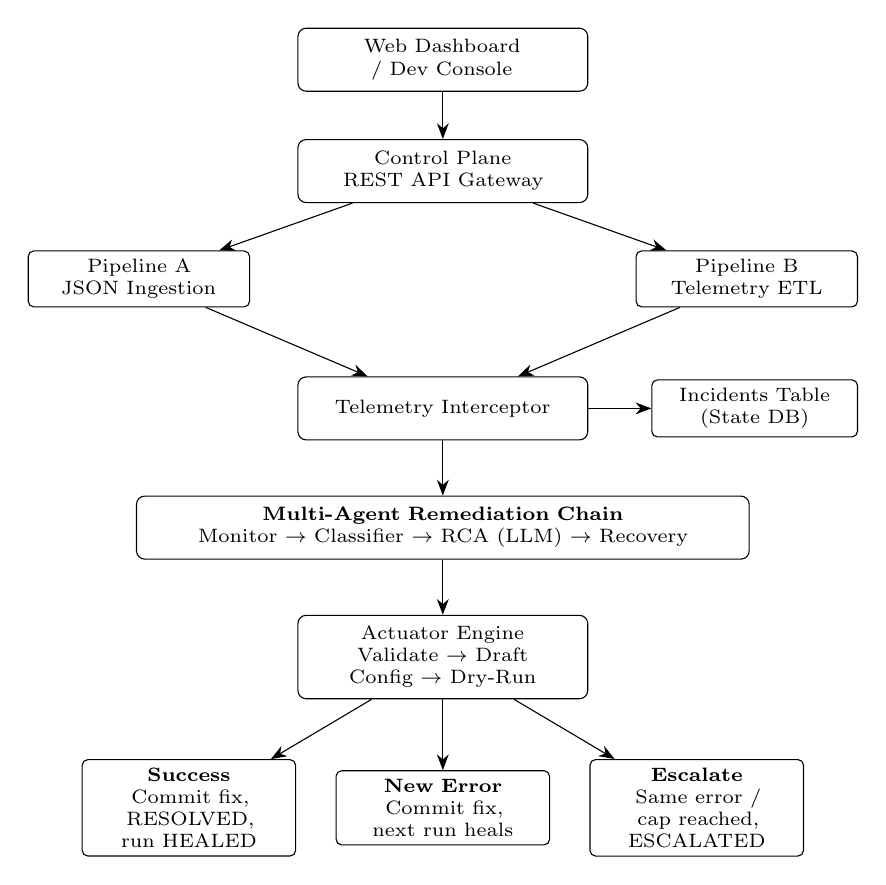
\begin{tikzpicture}[
  node distance=6mm and 10mm,
  every node/.style={font=\scriptsize},
  box/.style={draw=black, rounded corners=3pt, align=center, minimum height=8mm, inner sep=4pt, text width=3.4cm},
  tbox/.style={draw=black, rounded corners=2pt, align=center, minimum height=7mm, inner sep=3pt, text width=2.6cm},
  widebox/.style={draw=black, rounded corners=3pt, align=center, minimum height=8mm, inner sep=4pt, text width=7.5cm},
  arr/.style={-{Stealth[length=2mm]}, thin, draw=black}
]
% Row 1: UI
\node[box] (ui) {Web Dashboard / Dev Console};

% Row 2: API Gateway
\node[box, below=6mm of ui] (api) {Control Plane\\REST API Gateway};

% Row 3: Pipelines A & B side-by-side
\node[tbox, below left=6mm and 6mm of api] (pa) {Pipeline A\\JSON Ingestion};
\node[tbox, below right=6mm and 6mm of api] (pb) {Pipeline B\\Telemetry ETL};

% Row 4: Telemetry Interceptor & Incidents DB
\node[box, below=22mm of api] (tel) {Telemetry Interceptor};
\node[tbox, right=8mm of tel, text width=2.4cm] (inc) {Incidents Table\\(State DB)};

% Row 5: Multi-Agent Remediation Chain
\node[widebox, below=7mm of tel] (lg) {\textbf{Multi-Agent Remediation Chain}\\Monitor $\rightarrow$ Classifier $\rightarrow$ RCA (LLM) $\rightarrow$ Recovery};

% Row 6: Actuator Engine
\node[box, below=7mm of lg] (act) {Actuator Engine\\Validate $\rightarrow$ Draft Config $\rightarrow$ Dry-Run};

% Row 7: Outcome Branches
\node[tbox, below=9mm of act, text width=2.5cm] (it) {\textbf{New Error}\\Commit fix, next run heals};
\node[tbox, left=5mm of it, text width=2.5cm] (ok) {\textbf{Success}\\Commit fix, RESOLVED, run HEALED};
\node[tbox, right=5mm of it, text width=2.5cm] (esc) {\textbf{Escalate}\\Same error / cap reached, ESCALATED};

% Connections
\draw[arr] (ui) -- (api);
\draw[arr] (api) -- (pa);
\draw[arr] (api) -- (pb);
\draw[arr] (pa) -- (tel);
\draw[arr] (pb) -- (tel);
\draw[arr] (tel) -- (inc);
\draw[arr] (tel) -- (lg);
\draw[arr] (lg) -- (act);
\draw[arr] (act) -- (ok);
\draw[arr] (act) -- (it);
\draw[arr] (act) -- (esc);
\end{tikzpicture}
\caption{Three-tier architecture: Data Plane, Control Plane, and the multi-agent remediation loop with its dry-run decision branch.}
\end{figure}

\subsection{Component Interaction Flow}
The lifecycle of an incident follows an explicit state machine managed by \code{IncidentManager.\_VALID\_TRANSITIONS}. Incidents start in an \code{OPEN} state, transition to \code{INVESTIGATING} during monitoring, move to \code{RCA\_COMPLETED} after root-cause analysis, proceed to \code{RECOVERY\_IN\_PROGRESS} when building a fix, and terminate at either \code{RESOLVED} or \code{ESCALATED} based on dry-run verification. Unsanctioned state jumps trigger a \code{RuntimeError}, safeguarding the system against invalid lifecycle state updates.

\begin{figure}[h]
\centering
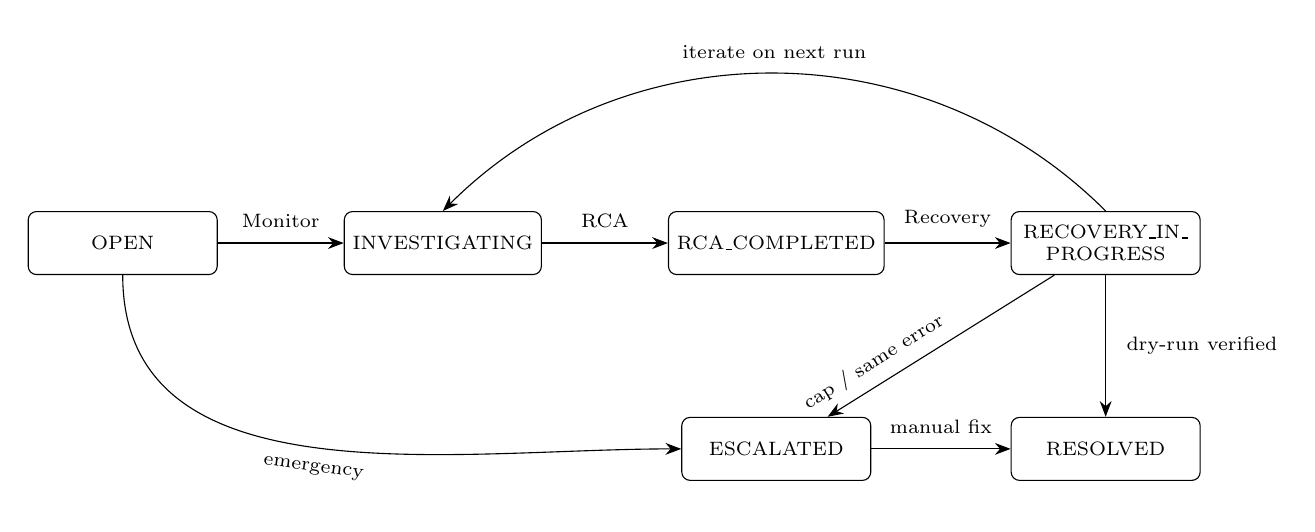
\begin{tikzpicture}[
  every node/.style={font=\scriptsize},
  st/.style={draw=black, rounded corners=3pt, minimum width=2.4cm, minimum height=8mm, align=center, inner sep=3pt},
  arr/.style={-{Stealth[length=2mm]}, thin, draw=black}
]
% Top Row: Active Lifecycle States
\node[st] (open) {OPEN};
\node[st, right=16mm of open] (inv) {INVESTIGATING};
\node[st, right=16mm of inv] (rca) {RCA\_COMPLETED};
\node[st, right=16mm of rca] (rec) {RECOVERY\_IN\_\\PROGRESS};

% Bottom Row: Terminal States
\node[st, below=18mm of rca] (esc) {ESCALATED};
\node[st, below=18mm of rec] (res) {RESOLVED};

% Top Row Transitions
\draw[arr] (open) -- node[above=2pt]{Monitor} (inv);
\draw[arr] (inv) -- node[above=2pt]{RCA} (rca);
\draw[arr] (rca) -- node[above=2pt]{Recovery} (rec);

% Resolution & Escalation Branches
\draw[arr] (rec) -- node[right=4pt]{dry-run verified} (res);
\draw[arr] (rec) -- node[pos=0.4, above left=1pt, sloped]{cap / same error} (esc);
\draw[arr] (esc) -- node[above=2pt]{manual fix} (res);

% Secondary Arc Paths
\draw[arr] (open.south) to[out=-90, in=180] node[below=2pt, sloped]{emergency} (esc.west);
\draw[arr] (rec.north) to[out=135, in=45] node[above=2pt]{iterate on next run} (inv.north);
\end{tikzpicture}
\caption{Incident lifecycle state machine, enforced in \code{src/incidents/incident\_manager.py}.}
\end{figure}

% =====================================================
\section{Core Deterministic Modules}
To optimize performance and minimize API overhead, the platform relies heavily on deterministic components. LLM calls are reserved exclusively for generating diagnostic summaries or resolving structural ambiguities that rule-based logic cannot settle.

\subsection{Structural and Type Validation}
Pipeline A uses a typed \code{CustomerRecord} model (\code{src/pipeline/json\_pipeline.py}) to validate every incoming record before writing to the database. Field validators handle type coercion (for example, converting integer \code{5} into string \code{"5"}), enforce non-empty primary keys, and check email formatting. Validation errors are accumulated per row, allowing valid records to proceed while isolating invalid entries.

\subsection{Structured Error Signatures}
When a pipeline encounters a failure, it generates a hash-based error signature (e.g., \code{[ErrorSignature: PIPELINE\_A|KeyError|country|dfe5f9c7e9420155]}) using \code{generate\_error\_signature()} in \code{src/config.py}. This signature provides the recovery agent with precise, structured context and serves as a key in the database configuration table, enabling verified fixes to be reused automatically on future runs.

\subsection{Severity and Category Classification}
The \code{SeverityRulesEngine} (\code{src/incidents/severity\_rules.py}) classifies incoming exceptions into categories (\code{SCHEMA\_DRIFT}, \code{DATA\_QUALITY}, \code{NETWORK\_TIMEOUT}, etc.) and assigns severity levels (\code{P0} through \code{P3}). This classification runs deterministically prior to agent invocation, ensuring critical system crashes immediately route to \code{P0} while minor record defects map to \code{P3}.

\subsection{Deterministic Schema-Drift Resolution}
Schema renames are handled primarily through alias mapping and fuzzy string matching in \code{src/agents/recovery.py}. Configuration settings in \code{configs/settings.yaml} define known column aliases (e.g., \code{country\_col} accepting \code{country}, \code{nation}, \code{region}, or \code{geo}). When a missing field is detected, \code{\_resolve\_param\_name} and \code{\_best\_fuzzy\_match} (\code{difflib.SequenceMatcher}) compare the missing key against payload fields. If a match is found above the similarity threshold, the field mapping is updated without invoking an LLM.

\subsection{Safety Guards and Hybrid Quarantine}
Proposed fixes undergo validation in \code{RemediationService.validate\_fix\_schema} to check parameter keys against an approved whitelist, enforce alphanumeric value constraints, and guard against SQL injection patterns (\code{drop}, \code{union}, \code{delete}, etc.). Meanwhile, row-level validation errors are captured by \code{QuarantineService} and stored in a \code{quarantined\_records} table. The pipeline run finishes with a \code{QUARANTINED} status and logs an auto-resolved \code{P3} warning incident. If an entire batch fails validation, the pipeline raises a full error, triggering agentic remediation.

% =====================================================
\section{Multi-Agent Remediation Pipeline}

\subsection{Agent Design: A Linear, Deterministic-First Chain}
The remediation workflow (\code{src/orchestration/graph.py}) executes as a sequential four-node graph: \textbf{Monitor}, \textbf{Classifier}, \textbf{RCA}, and \textbf{Recovery}. 
\begin{itemize}
  \item \textbf{Monitor}: Normalizes incoming telemetry and updates incident status.
  \item \textbf{Classifier}: Evaluates blast radius and escalates severity to \code{P0} if multiple unresolved incidents exist for the pipeline.
  \item \textbf{RCA}: Invokes the LLM to generate a clear, technical root-cause analysis (with a hardcoded fallback string in case of API timeouts).
  \item \textbf{Recovery}: Executes deterministic alias resolution first, falling back to LLM key-matching or query rewriting only if deterministic methods fail.
\end{itemize}

\subsection{Verification by Execution, Not Opinions}
Rather than relying on a secondary agent to critique proposed remedies, the system uses empirical validation. In \code{RemediationService.\_handle\_reconfigure}, the proposed change is saved as an \emph{unverified draft} configuration. The pipeline is then rerun against the source dataset in a dry-run mode (\code{throw\_on\_error=True}):
\begin{itemize}
  \item \textbf{Dry-Run Succeeds}: The draft configuration is verified, the run is marked \code{HEALED}, and the incident transitions to \code{RESOLVED}.
  \item \textbf{New Structural Error Appears}: Indicates the initial drift was resolved; the fix is saved, and the remaining drift is left for the next run.
  \item \textbf{Original Error Persists}: The draft is discarded, and the incident escalates to human engineers.
\end{itemize}

\subsection{Decision Model and Circuit Breaker}
The platform employs discrete state transitions and severity levels rather than continuous numerical scoring. To prevent runaway loops during compounding failure modes, a circuit breaker (\code{RemediationService.MAX\_HEAL\_ATTEMPTS = 4}) caps the maximum number of automated healing attempts per pipeline run. If the attempt threshold is reached, the system halts automated retries and escalates the issue.

\subsection{LLM Backend}
LLM-based tasks utilize a high-performance Flash-tier model configured in \code{configs/settings.yaml} with \code{temperature: 0.0}, a 10-second timeout, and 3 automatic retries. Structured JSON outputs are enforced using Pydantic schemas. If API rate limits (HTTP 429) are encountered, the system gracefully escalates the incident for manual intervention.

% =====================================================
\section{API Design and Endpoints}
The Control Plane provides a REST API interface implemented in \code{src/api/main.py}:

\begin{center}
\small
\begin{tabularx}{\textwidth}{@{}l X@{}}
\toprule
\textbf{Endpoint} & \textbf{Purpose} \\
\midrule
\code{POST /telemetry/incident} & Receives failure telemetry, initializes an incident, and triggers asynchronous remediation. \\
\code{POST /api/pipelines/a/execute} & Executes Pipeline A against sample test files or uploaded JSON data, returning status and ingestion counts. \\
\code{POST /api/pipelines/b/execute} & Executes Pipeline B against test databases or uploaded SQLite files. \\
\code{GET /api/metrics} & Fetches system-wide metrics (resolved, investigating, escalated, quarantined, and clean runs). \\
\code{GET /api/incidents} & Retrieves all registered incidents, sorted chronologically. \\
\code{GET /api/incidents/\{incident\_id\}/audit} & Fetches detailed audit logs for a given incident ID. \\
\code{GET /api/quarantine} & Retrieves quarantined records along with their validation error messages. \\
\code{GET /api/escalations} & Reads human escalation logs from \code{escalated\_incidents.log}. \\
\code{POST /api/history/clear} & Resets database tables and history to a baseline state. \\
\code{POST /runs/register}, \code{POST /runs/\{run\_id\}/status} & Internal endpoints for tracking pipeline execution runs. \\
\bottomrule
\end{tabularx}
\end{center}

% =====================================================
\section{Web Interface}
The platform provides two UI interfaces:
\begin{enumerate}
  \item \textbf{Web Dashboard}: A static single-page application (\code{public/index.html} and \code{public/app.js}) built with utility CSS and served by the API server. It features an interactive sandbox for testing pipeline executions, real-time incident tracking (polling every 3 seconds), quarantine inspection panels, and audit log views.
  \item \textbf{Development Console}: A secondary dashboard (\code{src/ui/app.py}) for local testing, equipped with real-time state refresh widgets (\code{st.fragment}).
\end{enumerate}

\begin{figure}[h]
\centering
\fbox{\parbox{0.85\linewidth}{\centering\vspace{1.6cm}
Figure placeholder: Operations Dashboard in clean baseline state (\code{python run\_platform.py}).
\vspace{1.6cm}}}
\caption{Dashboard baseline state (placeholder).}
\end{figure}

\begin{figure}[h]
\centering
\fbox{\parbox{0.85\linewidth}{\centering\vspace{1.6cm}
Figure placeholder: Active incident undergoing automated remediation and dry-run verification.
\vspace{1.6cm}}}
\caption{Active incident during remediation (placeholder).}
\end{figure}

\begin{figure}[h]
\centering
\fbox{\parbox{0.85\linewidth}{\centering\vspace{1.6cm}
Figure placeholder: Comparison view showing RESOLVED incident alongside an ESCALATED log entry.
\vspace{1.6cm}}}
\caption{Resolved vs. Escalated incident views (placeholder).}
\end{figure}

% =====================================================
\section{Deployment}

\subsection{Cloud Serverless Configuration and Dual-Database Adapter}
The codebase includes serverless routing configuration (\code{vercel.json}) pointing to a single function entrypoint (\code{src/api/main.py}). Because serverless environments use temporary filesystems, \code{src/database.py} includes an adapter layer: when a \code{POSTGRES\_URL} environment variable is present, SQL queries automatically adjust placeholder syntax (\code{?} to \code{\%s}) and translate \code{INSERT OR REPLACE} statements into PostgreSQL \code{ON CONFLICT} upserts. API credentials and database strings are managed through environment variables.

\subsection{Current Deployment Status}
The platform is deployed live on Vercel serverless cloud hosting at \url{https://enterprise-data-pipeline-orchestrat.vercel.app/}. All REST endpoints (\code{/api/metrics}, \code{/api/incidents}, \code{/api/quarantine}, \code{/api/escalations}) and pipeline execution sandbox controllers are fully operational, handling live data ingestion, autonomous multi-agent remediation, and quarantine logging in a production serverless runtime.

% =====================================================
\section{Testing and Validation}

\subsection{Sample Execution: Single-Column Schema Drift (Verified)}
Running \code{test\_data/pipeline\_A/case\_drift\_country.json} (where \code{country} is renamed to \code{nation}) through \code{POST /api/pipelines/a/execute} yields the following execution trace:

\begin{logblock}
error="[ErrorSignature: PIPELINE\_A|KeyError|country|dfe5f9c7e9420155] Expected: ['customer\_id', 'name', 'email', 'country'] | Found: [..., 'nation']"\\
...\\
Final remediation vector: \{'action': 'RECONFIGURE', 'params': \{'country\_col': 'nation'\}, ...\}\\
...\\
Pipeline dry-run succeeded; committing config version\\
Incident state shifted: RECOVERY\_IN\_PROGRESS -> RESOLVED\\[4pt]
API response: \{'status': 'success', 'rows\_ingested': 'Auto-healed', 'healed': True\}\\
pipeline\_runs: [('run\_a\_e6203d', 'HEALED')]\\
incidents:     [('RESOLVED', 'SCHEMA\_DRIFT', 'P1')]\\
customers ingested: 10
\end{logblock}

The deterministic matcher successfully mapped \code{nation} to \code{country\_col} without relying on an LLM for the mapping logic. The dry-run verified the fix, ingested 10 rows, and committed the override.

\subsection{Edge Case: Multi-Column Drift \& Recursion Bug Resolution (Verified)}
Testing multi-column drift (\code{case\_drift\_multi.json}, containing simultaneous \code{customer\_id $\rightarrow$ id} and \code{email $\rightarrow$ user\_email} drifts) revealed an initial defect: the recovery agent alternated between resolving individual column errors, causing dry-runs to clear previous overrides and entering an infinite loop.

This was resolved by:
\begin{enumerate}
  \item Preventing dry-run executions from re-triggering nested telemetry incidents (\code{throw\_on\_error=True}).
  \item Implementing a \code{MAX\_HEAL\_ATTEMPTS = 4} circuit breaker.
\end{enumerate}

Following the fix, the pipeline successfully converges over two sequential passes:
\begin{logblock}
Run 1: \{'status': 'success', 'rows\_ingested': 'Auto-healed', 'healed': True\} \quad customers: 0\\
Run 2: \{'status': 'success', 'rows\_ingested': 'Auto-healed', 'healed': True\} \quad customers: 10\\[4pt]
Total incidents logged: 2 (previously infinite)
\end{logblock}

\subsection{Regression Testing: Baseline Configuration Reset (Verified)}
To ensure committed overrides do not corrupt future healthy runs, post-heal baseline resetting was refactored so overrides reset only after full execution success. Running \code{case\_healthy.json} after healing a drift file successfully ingested 10 rows without leftover configuration artifacts.

\subsection{Automated Test Suite Results (Verified)}
The test suite in \code{test/test\_recovery.py} was executed to verify core recovery and validation behavior:

\begin{logblock}
test/test\_recovery.py::test\_best\_fuzzy\_match\_and\_resolve PASSED\\
test/test\_recovery.py::test\_recovery\_agent\_node\_schema\_drift PASSED\\
test/test\_recovery.py::test\_remediation\_service\_validate\_fuzzy\_accept PASSED\\
test/test\_recovery.py::test\_remediation\_service\_rejects\_unknown PASSED\\
test/test\_recovery.py::test\_alias\_not\_in\_payload\_should\_escalate PASSED\\
test/test\_recovery.py::test\_alias\_in\_payload\_matches\_alias\_to\_param PASSED\\
test/test\_recovery.py::test\_llm\_fallback\_aligns\_to\_found\_key PASSED\\
test/test\_recovery.py::test\_pipeline\_b\_allows\_sql\_override PASSED\\
test/test\_recovery.py::test\_pipeline\_a\_rejects\_sql\_in\_value PASSED\\
test/test\_recovery.py::test\_flatten\_root\_dict\_validation PASSED\\[4pt]
10 passed in 4.90s
\end{logblock}

% =====================================================
\section{Limitations and Future Work}

\subsection{Defects Resolved During Development}
Three primary issues were identified and fixed in commit \code{1a13bc83} on \code{main}:
\begin{enumerate}
  \item \textbf{Status Reporting Error}: Successful reconfigurations resolved incidents but failed to mark pipeline runs as \code{HEALED}. Fixed by updating run status flags upon verification.
  \item \textbf{Infinite Self-Healing Recursion}: Resolved by disabling nested telemetry triggers during dry-runs and introducing attempt thresholds.
  \item \textbf{Premature Config Reset}: Moved baseline reset calls to the actuator's confirmed success stage.
\end{enumerate}

\subsection{Known Open Limitations}
\begin{itemize}
  \item \textbf{Multi-Pass Convergence}: Multiple simultaneous column drifts resolve across sequential executions rather than in a single pass.
  \item \textbf{Discrete State Model}: The platform uses discrete severity levels and lifecycle states rather than continuous health scores.
  \item \textbf{Scope Boundary}: Focus is placed on data ingestion integrity rather than application code auditing or dependency vulnerabilities.
  \item \textbf{CDN Dependencies}: The default web interface references external CSS and font CDNs, requiring internet connectivity for full styling.
\end{itemize}

\subsection{Future Work}
\begin{itemize}
  \item Enhance the actuator to resolve multi-column drifts within a single dry-run pass.
  \item Introduce an optional rolling pipeline reliability index alongside discrete state tracking.
  \item Vendor static CSS assets and fonts locally to support fully offline environments.
  \item Complete cloud deployment with managed database integration.
\end{itemize}

% =====================================================
\section{Conclusion}
This project demonstrates an agentic, self-healing data pipeline platform combining deterministic schema recovery, a structured multi-agent workflow, and empirical dry-run verification. By isolating row-level anomalies into quarantine and validating fixes against live execution, the system maintains high ingestion availability while preventing corrupt data writes. Key recursion and status reporting bugs discovered during multi-column drift testing were resolved and verified against unit tests, establishing a reliable foundation for automated data operations.

\bigskip
\noindent\rule{\textwidth}{0.4pt}

\footnotesize
All system details, API schemas, and test outputs presented in this report were verified against repository commit \code{2f760d9f} on \code{main}.

\end{document}
